\begin{figure}[!h]
\centering
\resizebox{\textwidth}{!}{%
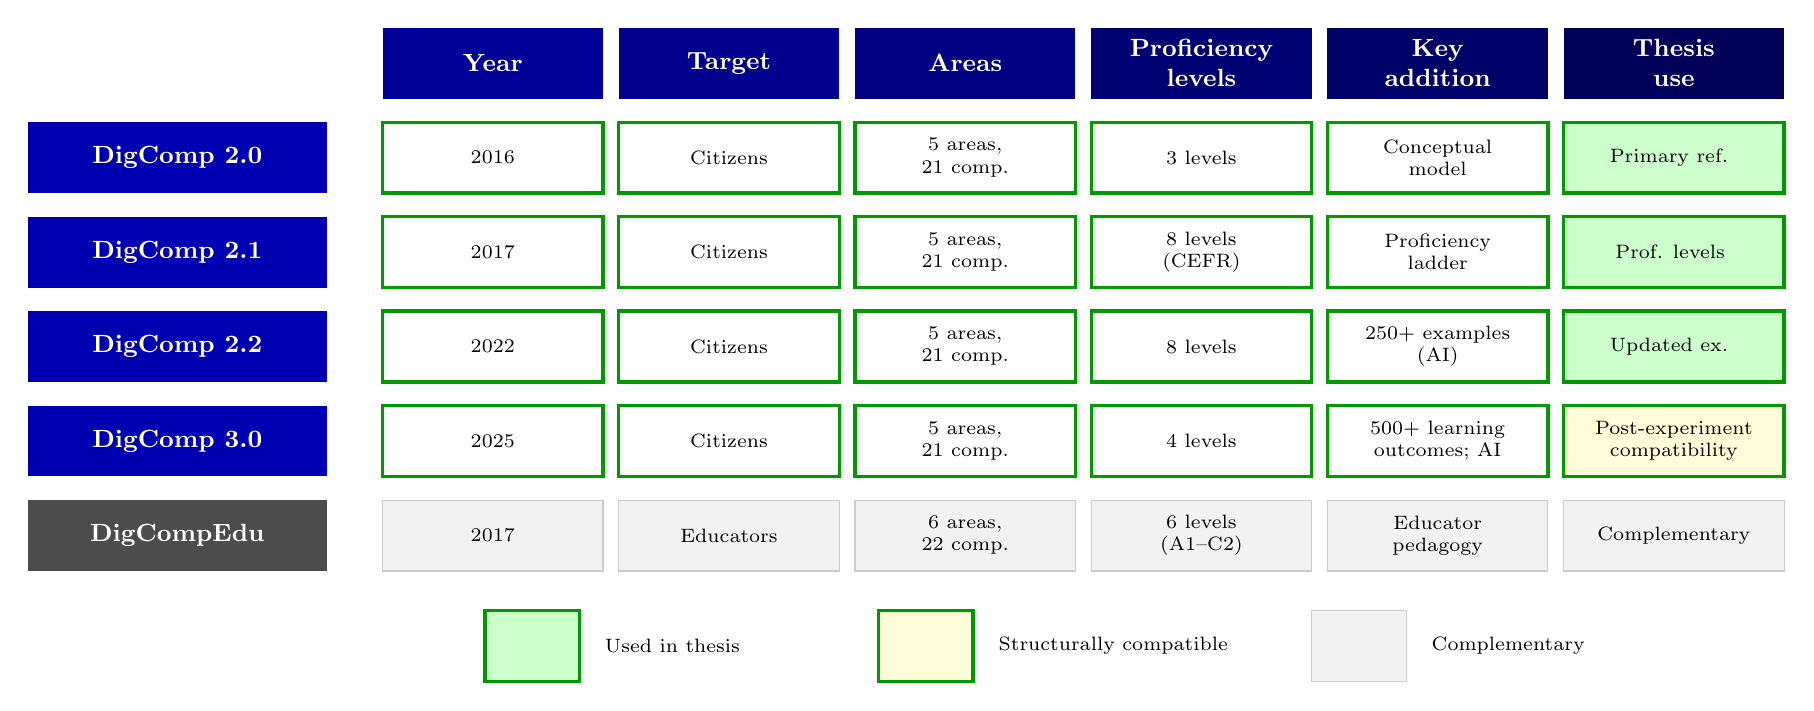
\begin{tikzpicture}[
  hdr/.style={font=\small\bfseries, text=white, minimum height=0.9cm,
    minimum width=2.8cm, align=center},
  rhdr/.style={font=\small\bfseries, text=white, minimum height=0.9cm,
    minimum width=3.8cm, align=center, anchor=east},
  cell/.style={rectangle, draw=gray!40, minimum height=0.9cm,
    minimum width=2.8cm, align=center, font=\scriptsize},
  usedcell/.style={cell, draw=green!60!black, line width=1.2pt},
  graycell/.style={cell, fill=gray!10},
  usedr/.style={font=\small\bfseries, text=white, minimum height=0.9cm,
    minimum width=3.8cm, align=center, anchor=east, fill=blue!70!black},
  grayr/.style={font=\small\bfseries, text=white, minimum height=0.9cm,
    minimum width=3.8cm, align=center, anchor=east, fill=gray!60!black},
]

% Column spacing
\def\colw{3.0}

% Column headers
\node[hdr, fill=blue!60!black] at (0, 0) {Year};
\node[hdr, fill=blue!55!black] at (\colw, 0) {Target};
\node[hdr, fill=blue!50!black] at (2*\colw, 0) {Areas};
\node[hdr, fill=blue!45!black] at (3*\colw, 0) {Proficiency\\levels};
\node[hdr, fill=blue!40!black] at (4*\colw, 0) {Key\\addition};
\node[hdr, fill=blue!35!black] at (5*\colw, 0) {Thesis\\use};

% Row 1: DigComp 2.0 — used in thesis (green border)
\node[usedr] at (-2.1, -1.2) {DigComp 2.0};
\node[usedcell] at (0, -1.2) {2016};
\node[usedcell] at (\colw, -1.2) {Citizens};
\node[usedcell] at (2*\colw, -1.2) {5 areas,\\21 comp.};
\node[usedcell] at (3*\colw, -1.2) {3 levels};
\node[usedcell] at (4*\colw, -1.2) {Conceptual\\model};
\node[usedcell, fill=green!20] at (5*\colw, -1.2) {Primary ref. \checkmark};

% Row 2: DigComp 2.1 — used in thesis (green border)
\node[usedr] at (-2.1, -2.4) {DigComp 2.1};
\node[usedcell] at (0, -2.4) {2017};
\node[usedcell] at (\colw, -2.4) {Citizens};
\node[usedcell] at (2*\colw, -2.4) {5 areas,\\21 comp.};
\node[usedcell] at (3*\colw, -2.4) {8 levels\\(CEFR)};
\node[usedcell] at (4*\colw, -2.4) {Proficiency\\ladder};
\node[usedcell, fill=green!20] at (5*\colw, -2.4) {Prof. levels \checkmark};

% Row 3: DigComp 2.2 — used in thesis (green border)
\node[usedr] at (-2.1, -3.6) {DigComp 2.2};
\node[usedcell] at (0, -3.6) {2022};
\node[usedcell] at (\colw, -3.6) {Citizens};
\node[usedcell] at (2*\colw, -3.6) {5 areas,\\21 comp.};
\node[usedcell] at (3*\colw, -3.6) {8 levels};
\node[usedcell] at (4*\colw, -3.6) {250+ examples\\(AI)};
\node[usedcell, fill=green!20] at (5*\colw, -3.6) {Updated ex. \checkmark};

% Row 4: DigComp 3.0 — contextual (green border, published after experiment)
\node[usedr] at (-2.1, -4.8) {DigComp 3.0};
\node[usedcell] at (0, -4.8) {2025};
\node[usedcell] at (\colw, -4.8) {Citizens};
\node[usedcell] at (2*\colw, -4.8) {5 areas,\\21 comp.};
\node[usedcell] at (3*\colw, -4.8) {4 levels};
\node[usedcell] at (4*\colw, -4.8) {500+ learning\\outcomes; AI};
\node[usedcell, fill=yellow!15] at (5*\colw, -4.8) {Post-experiment\\compatibility};

% Row 5: DigCompEdu — complementary (gray)
\node[grayr] at (-2.1, -6.0) {DigCompEdu};
\node[graycell] at (0, -6.0) {2017};
\node[graycell] at (\colw, -6.0) {Educators};
\node[graycell] at (2*\colw, -6.0) {6 areas,\\22 comp.};
\node[graycell] at (3*\colw, -6.0) {6 levels\\(A1--C2)};
\node[graycell] at (4*\colw, -6.0) {Educator\\pedagogy};
\node[graycell] at (5*\colw, -6.0) {Complementary};

% Legend
\node[usedcell, fill=green!20, minimum width=1.2cm] at (0.5, -7.4) {};
\node[font=\scriptsize, anchor=west] at (1.3, -7.4) {Used in thesis};
\node[usedcell, fill=yellow!15, minimum width=1.2cm] at (5.5, -7.4) {};
\node[font=\scriptsize, anchor=west] at (6.3, -7.4) {Structurally compatible};
\node[graycell, minimum width=1.2cm] at (11.0, -7.4) {};
\node[font=\scriptsize, anchor=west] at (11.8, -7.4) {Complementary};

\end{tikzpicture}%
}% end resizebox
\caption{The DigComp framework family: evolution and application in this thesis. All DigComp versions maintain the same five-area, 21-competence structure; differences lie in proficiency granularity, illustrative examples, and --- in DigComp~3.0 --- learning outcomes and AI integration. DigCompEdu addresses educator-specific competences and is used as a complementary reference. This thesis uses DigComp~2.0 as the primary conceptual framework (consistent with \citeauthor{Titova2025cte}~\cite{Titova2025cte}), with proficiency levels from DigComp~2.1 and updated examples from DigComp~2.2. DigComp~3.0 \citep{Cosgrove2025}, published after the experimental study, is structurally compatible with the thesis findings (see Section~\ref{sec:digcomp}).}
\label{fig:digcomp-framework-landscape}
\end{figure}
